\documentclass[10pt,twocolumn,letterpaper]{article} 

\usepackage{cvpr}
\usepackage{times}
\usepackage{epsfig}
\usepackage{graphicx}
\usepackage{amsmath}
\usepackage[psamsfonts]{amssymb}
\usepackage{url}

\def\RR{\mathbb{R}}
\def\NN{\mathbb{N}}
\def\xx{\mathbf{x}}
\def\ww{\mathbf{w}}
\def\aa{\mathbf{\alpha}}
\def\bb{\mathbf{\beta}}
\def\ee{\mathbf{e}}
\def\dd{\mathbf{d}}
\def\mdd{\tilde{\dd}}
\def\b{\mathcal{B}}
\def\d{\mathcal{D}}

% ------------------------------------------------------------------------ 

% Include other packages here, before hyperref.

\usepackage[pagebackref=true,breaklinks=true,letterpaper=true,colorlinks,bookmarks=false]{hyperref}
% \cvprfinalcopy % *** Uncomment this line for the final submission
\def\cvprPaperID{****} % *** Enter the CVPR Paper ID here
\def\httilde{\mbox{\tt\raisebox{-.5ex}{\symbol{126}}}}
\ifcvprfinal\pagestyle{empty}\fi

\begin{document}

% ------------------------------------------------------------------------ 

\title{Online place recognition in complex robot navigation \\
using reduced-rank support vector classification}

\author{Francesco Orabona\\
LIRA-Lab, University of Genova\\
viale F. Causa, 13, 16145 Genova, Italy\\
{\tt\small bremen@liralab.it}
% For a paper whose authors are all at the same institution, 
% omit the following lines up until the closing ``}''.
% Additional authors and addresses can be added with ``\and'', 
% just like the second author.
% To save space, use either the email address or home page, not both
\and
Second Author\\
Institution2\\
First line of institution2 address\\
{\small\url{http://www.author.org/~second}}
}

\maketitle
% \thispagestyle{empty}

% ------------------------------------------------------------------------ 

\begin{abstract}
Grasping is one of the most challenging tasks in advanced robotics...

\end{abstract}

% ------------------------------------------------------------------------ 
%%%%%%%%%%%%%%%%%%%%%%%%%%%%%%%%%%%%%%5
\section{Introduction}
\label{introduction}
%%%%%%%%%%%%%%%%%%%%%%%%%%%%%%%%%%%%%%
Consider Figure \ref{fig:chairs}, representing $(a)$ a chair, and $(b)$ Santiago
Calatrava's ``sedia redonda'', the round chair, a particularly stylish object of
design sold as a chair in the Sixties. What makes us claim that these objects
both belong to the category of chairs? Indeed, this is an ominous problem in
object recognition: too often the category of an object is determined by its
function rather than by its visual appearance alone. The very concept of object
has been re-defined by Gibson \cite{gibson} in terms of its affordances ---
``what one can do with it''. According to this view, what ties both the objects in
Figure \ref{fig:chairs} to the category of chairs is the fact that they are
used to sit down.

Further hints at a strong link between perception and action come from neuroscience,
in particular from the mirror neurons paradigm \cite{fadiga}. According to the
mirror theory, neural correlates are found for both the performance of a grasping
action (mainly involving the sensorimotor system of primates) and its visual
representation when performed by another primate (involving the visual system only).
If this is true, as it seems, then the monkeys' (and our) object classification is
so robust mainly because these biological systems \emph{know what to do} with the
objects they see --- a capability which machines lack, so far. Picture, for instance,
how much easier automated object recognition of a mug would be under changing illumination
conditions, if only our machine had an idea of how to grasp something which looked like
a mug.

Inspired by these considerations, we hereby define a theoretical framework for
reconstructing \emph{active} sensory modalities from \emph{passive} ones, that is in
short, for figuring out what to do with what one sees, hears, smells etc. In particular,
we enforce one such schema using a multi-variate regression technique to associate
\emph{object visual features} to related \emph{human grasping postures}. This schema is
called a \emph{Visuo-Motor Map} (VMM) and is trained
using a large database of visual and motor data collected from human subjects, that
we call the \emph{Visuo-Motor Grasping dataBase} (VMGdB). The immediate result is the
ability of retrieving a (set of) grasping posture(s) just by seeing an object; this
ability, which we call \emph{grasp priming}, has obvious applications in robotic fields
where (semi)autonomous grasping / fine manipulation is reuquired, such as robotic surgery,
humanoid robotics, teleoperation, advanced hand prosthetics etc.

Since, though, the focus of this work is on enhancing object reocgnition, we then show
that these grasping postures, reconstructed by the VMM, dramatically improve the
classification rate of a standard object classifier.

The paper is organised like this: in Section \ref{sec::framework} we define the general
multi-modal learning framework, and then we describe the instance under examination;
we then describe in detail the vision-related unit (Section \ref{sec::vision}) and the
regression schema employed to build the VMM (Section \ref{sec::regression}). We then show our
experimental results (Section \ref{sec::experiments}) and conclude in Section \ref{sec::concl}.

%\begin{itemize}
%
%\item learning by imitation great capability of cognitive systems. It permits to learn how to grasp a cup never seen before just by seeing someone else doing it.
%Fundamental learning mechanism etc 
%
%\item a widely accredited hip is that the underlying mechanism of learning by imitation is the existence of a sensor motor map that links
%the visual perception of an object to the motir position of the hand when it manipulates it. Mirror neurons blabla 
%
%\item another consequence of the existence of a sensor-motor map is that when we learn an object by seeing and manipulating it, we are then able
%to recognize it with a higher degree of accuracy and robustness than if we would have learned it on visual data only. 
%
%\item Enabling a robot to display similar abilities is one of the holy grails of research in artificial cognitive systems. 
%
%\item In this paper we present a mirror neurons inspired algorithm for building perception action maps between visual, passive perception and motor, active
%perception. During learning, the algorithm takes as input visual and sensomotor data and (a) it builds a mapping between the two modalities (b) it builds 
%a classifier on both modalities. After training, wehn presented with a visual input, the system is able to perform grasp priming (= is able to predict
%which are the possible way to grasp the seen object; this information could be used to pre-activate a robot hand) and enhanced visual recognition
%(= is able to recognize objects with a higher degree of accuracy and robustness compared to a model learned only on visual features, even if
%the sensor modality is not perceived by the agent). Experiments show that.....
%
%\item in the rest of the paper...
%
%\end{itemize}


%%%%%%%%%%%%%%%%%%%%%%%%%%%%%%%%%%%%%%%%
\section{Previous Work}
\label{prev-work}
%%%%%%%%%%%%%%%%%%%%%%%%%%%%%%%%%%%%%%%%
The exploitation of SVM solution sparseness probably appears first in
\cite{DownsGM01}: a simplification of the decision function is therein
proposed, based upon linear independence of the support vectors in the
feature space, performed \emph{after} the training is done. This is a
simple consequence of the fact that, if the feature space has
dimension $n$, at most $n+1$ independent SVs are required to build the
solution \cite{PontilV98}. Downs et al.'s idea is useful in reducing
the testing time, but not the training time, since every time new data
is available training must be performed from scratch and taking into
account all SVs found so far. Discarding from the sample set the
linearly dependent SVs won't work, unless one is prepared to lose
accuracy --- in fact, other methods to heuristically select a subset
of the support vectors have been proposed,
e.g. \cite{LeeM01,schoel06,KeerthiCDC06}.

In order to keep the solution compact without losing accuracy, the key
is to keep the size of the kernel matrix small, i.e., reducing its
rank. Unsupervised rank reduction methods have been proposed, e.g., in
\cite{KeerthiCDC06}, as well as supervised ones
\cite{Baudat03,BachJordan2005}, but no application of these ideas
appears so far, to the best of our knowledge, in online settings. This
is particularly important since it has been shown \cite{Steinwart03}
that the SV set grows linearly with the sample set; therefore, in an
online setting, a SVM would grow indefinitely.

The exact solution to online SVM learning was given by Cauwenberghs
and Poggio in 2000 \cite{CauwenberghsP00}, but their idea has received
little attention in the community so far \cite{Laskov2006}, probably
due to the lack of a detailed analysis of its complexity.



%%%%%%%%%%%%%%%%%%%%%%%%%%%%%%%%%%%%%%%%%%
\section{Background Mathematics}
\label{sec:bg}
%%%%%%%%%%%%%%%%%%%%%%%%%%%%%%%%%%%%%%%%%%
Due to space limitations, this is a very quick account of SVMs --- the
interested reader is referred to \cite{Burges98} for a tutorial, and
to \cite{Cristianini00} for a comprehensive introduction to the
subject. Assume $\{\xx_i,y_i\}_{i=1}^l$, with $\xx_i \in \RR^m$ and
$y_i \in \{-1,1\}$, is a set of samples and labels drawn from an
unknown probability distribution; we want to find a function $f(\xx)$
such that $sign(f(\xx))$ best determines the category of any future
sample $\xx$. In the most general setting,

\begin{equation} \label{eqn:sol}
  f(\xx) = \sum_{i=1}^l \alpha_i y_i K(\xx,\xx_i) + b
\end{equation}

\noindent where $b \in \RR$ and $K(\xx_1,\xx_2) = \Phi(\xx_1)
\cdot \Phi(\xx_2)$, the \emph{kernel function}, evaluates inner
products between images of the samples through a non-linear mapping
$\Phi$. The $\alpha_i$s are Lagrangian coefficients obtained by
solving (the dual Lagrangian form of) the problem

\begin{eqnarray} \label{eqn:svm_primal}
  \min_{\ww,b}      & \frac{1}{2} ||\ww||^2 + C \sum_{i=1}^l \xi_i^p            \\
  \mbox{subject to} & y_i (\ww\cdot\xx_i + b) \geq 1-\xi_i            \nonumber \\
                    & \xi_i \geq 0                                    \nonumber
\end{eqnarray}

\noindent where $\ww$ defines a separating hyperplane
in the \emph{feature space}, i.e., the space where $\Phi$ lives,
whereas $\xi_i \in \RR$ are slack variables, $C \in \RR^+$ is an error
penalty coefficient and $p$ is usually $1$ or $2$. In practice, most
of the $\alpha_i$ are found to be zero after training; the vectors
with an associated $\alpha_i$ different from zero are called
\emph{support vectors}. Notice that, from (\ref{eqn:sol}), the testing
time of a new point is proportional to the number of SVs, hence
reducing the number of SVs implies reducing the testing time.

In the following, the term \emph{kernel dimension} will refer, as is
customary, to the dimension of the feature space. The kernel dimension
is related to the generalization power of the machine, and it depends
on the choice of the kernel itself. Widely used kernels include the
\emph{polynomial} one (finite-dimensional) and the \emph{Gaussian} one
(infinite-dimensional).


%%%%%%%%%%%%%%%%%%%%%%%%%%%%%%%%%%%%%%%%%%
\section{Sparseness of the solution}
\label{sec:spars}
%%%%%%%%%%%%%%%%%%%%%%%%%%%%%%%%%%%%%%%%%%
The time required by an SVM to train and predict is, in turn, cubic
and linear in the number of support vectors
\cite{KeerthiCDC06}. Moreover, a recent result by Steinwart
\cite{Steinwart03} indicates that the number of support vectors, $r$,
increases linearly with the number $l$ of training samples. (Given a
kernel function $K$, $r$ tends to $2 B_K l$, where $B_K$ is the
smallest classification error achievable with the kernel $K$.)
Therefore, although support vectors somehow code all the information
required by the solution, their number grows indefinitely as the input
space is sampled. It is then highly desirable that the number of
support vectors is kept as small as possible, without losing accuracy.

Several ideas have been proposed to cope with this problem. One
possibility is that of heuristically choosing some support vectors,
thus obtaining an approximate solution, as is done, e.g., in
\cite{KeerthiCDC06,LeeM01,schoel06}. But if one is not willing to give
up exactness, then a strong hint on how to select support vectors
comes from the remark by Pontil and Verri \cite{PontilV98} that, if
the kernel has finite dimension $m$, at most $m + 1$ support vectors
are usually sufficient to fully determine the decision surface. This
idea is based upon linear independence in the feature space. In fact,
also in the case of infinitely-dimensional kernels, Downs et
al. \cite{DownsGM01} have shown that one can simplify the solution by
removing the linearly dependent support vectors, losing no
accuracy. Unfortunately, the simplification is therein performed
\emph{after} the training phase, so that it makes testing faster, but
not training.

In general, the possibility to obtain an alternative, possibly more
compact representation of the SVM solution follows from the fact that
the solution of a SVM problem is not unique if the
kernel matrix $K$, where $K_{ij} = K(\xx_i,\xx_j)$, does not have full
rank \cite{Burges98}, which is equivalent to some of the support vectors being
linearly dependent on the others \emph{in the feature space}. This
point can be confusing and needs an explanation: for instance, the
$\alpha_i$s obtained by Downs et al. in general do not respect the
Karush-Kuhn-Tucker (KKT) conditions --- a necessary condition for them
to be a solution to the SVM problem; but still they are equivalent to
the original optimal solution.

It turns out that this is exactly due to $K$ being
non-full-rank. Using the Representer Theorem
\cite{CoxOS90,KimeldorfW70}, Equation (\ref{eqn:w1}) can be written as
follows:

\begin{equation} \label{eqn:w2}
  \ww = \sum_{i=1}^l \beta_i \xx_i
\end{equation}

for a set of generic coefficients $\beta_i$. Substituting Equation
(\ref{eqn:w2}) in (\ref{eqn:lp1}) and using the kernel trick, we get

\begin{eqnarray} \label{eqn:svm_primal_general}
  L'_P =   \sum_{i,j}^l \left( \frac{1}{2}\beta_i-\alpha_i y_i \right) \beta_j K_{ij} \\
         - \sum_{i=1}^l \alpha_i (b y_i -1 +\xi_i) + \sum_{i=1}^l (C - \mu_i) \xi_i \nonumber
\end{eqnarray}

Now, enforcing the KKT conditions on \emph{this}, more general version
of the problem, one obtains that

\begin{equation} \label{eqn:kt2}
  \frac{\partial L'_P}{\partial \beta_i} = \sum_{i=1}^l (\beta_i - \alpha_i y_i) K_{ij} = 0
\end{equation}

Clearly, in order for (\ref{eqn:kt2}) to hold, the vector whose
components are $\beta_i-\alpha_i y_i$ must be in the null space of
$K$. Now if $K$ has full rank, the null space only consists of the
null vector, and therefore $\beta_i = \alpha_i y_i$ (this particular
result already appears in \cite{KeerthiCDC06}). Otherwise, there are
infinite solutions to the SVM problem, and the $\beta_i$s are not
constrained at all. This agrees with Downs et al.'s method, and the
very same result is obtained if we use the norm-2 formulation of
Equation (\ref{eqn:svm_primal}), that is, with $\sum_{i=1}^l \xi_i^2$.


%%%%%%%%%%%%%%%%%%%%%%%%%%%%%%%%%%%%%%%%%%%%%%%%%%%%%%%%%%%%%%%%%%%%%
\section{Incremental Independent Support Vector Classification}
\label{sec:opt}
%%%%%%%%%%%%%%%%%%%%%%%%%%%%%%%%%%%%%%%%%%%%%%%%%%%%%%%%%%%%%%%%%%%%%
Let the \emph{kernel matrix} $K$ be defined such that $K_{ij} =
K(\xx_i,\xx_j)$, with $i,j=1,\ldots,l$. The possibility to obtain a more
compact representation of $f(\xx)$ follows from the fact that the
solution to a SVM problem (that is, the $\alpha_i$s) is not unique if
$K$ does not have full rank \cite{Burges98}, which is equivalent to
some of the SVs being linearly dependent on some others \emph{in the
feature space} (this is the core of Downs et al.'s \cite{DownsGM01}
original idea).
Applying the idea of Downs et al., or any other post-training
method to reduce the number of SVs, in an online setting means simplifying the
solution each time a new sample is acquired, that is obviously infeasible.
We need a way to use independent SVs only, that is to
decouple the concept of ``basis'' vectors, used to build
the classification function (\ref{eqn:sol}), from the samples
used to evaluate the errors $\xi_i$ in (\ref{eqn:svm_primal}).
If the selected basis vectors span the same subspace as
the whole sample set, the solution found will be equivalent
--- that is, we will not lose any precision.

We hereby propose, after having received a new training sample, to
incrementally add it to the basis if it is linearly independent in the
feature space from those already present in the basis itself. The
solution found is \emph{the same} as in the classical SVM formulation;
therefore, no approximation whatsoever is involved, unless one gives
it up in order to obtain even fewer support vectors (see Section
\ref{sec:exp} for a deeper discussion on this point).

Denoting the indexes of the vectors in the current basis, after $l$
training samples, by $\b$, and the new sample under judgment by
$\xx_{l+1}$, the algorithm can then be summed up as follows:

\begin{enumerate}

  \item check whether $\xx_{l+1}$ is linearly independent from the
        basis in the feature space; if it is, add it to $\b$;
        otherwise, leave $\b$ unchanged.

  \item incrementally re-train the machine.

\end{enumerate}

Hence the testing time for a new point will be $O(|\b|)$.

In the following, the notations $A_{IJ}$ and $\mathbf{v}_I$, where $A$
is a matrix, $\mathbf{v}$ is a vector and $I,J \subset \NN$ denote in
turn the sub-matrix and the sub-vector obtained from $A$ and
$\mathbf{v}$ by taking the indexes in $I$ and $J$.

\subsection{Linear independence}

In general, checking whether a matrix has full rank is done via some
decomposition, or by looking at the eigenvalues of the matrix; but
here we want to check whether a \emph{single} vector is linearly
independent from a matrix which is already known to be
full-rank. Inspired by the definition of linear independence, we check
how well the vector can be approximated by a linear combination of the
vectors in the set \cite{EngelMM02sparse}. Let $d_j \in \RR$; then let

\begin{equation} \label{eqn:ald1}
  \Delta = \min_\dd \left|\left|\sum_{j \in \b} d_j \phi(\xx_j) - \phi(\xx_{l+1}) \right|\right|^2
\end{equation}

If $\Delta > 0$ then $\xx_{l+1}$ is linearly independent with respect
to the basis, and $\left\{l+1\right\}$ is added to $\b$. In practice, we check
whether $\Delta \leq \eta$ where $\eta > 0$ is a tolerance factor, and
expect that larger values of $\eta$ lead to worse accuracy, but also
to smaller bases. As a matter of fact, if $\eta$ is set at machine
precision, OISVMs retain the exact accuracy of SVMs. Notice also that
if the feature space has finite dimension $n$, then no more than $n$
linearly independent vectors can be found, and $\b$ will never contain
more than $n$ vectors.

Expanding equation (\ref{eqn:ald1}) we get

\begin{equation} \label{eqn:ald2}
  \Delta = \min_{\dd} \left( \sum_{i,j \in \b} d_j d_i \phi(\xx_j) \cdot \phi(\xx_i) 
    - 2\sum_{j \in \b} d_j \phi(\xx_j) \cdot \phi(\xx_{l+1})
    + \phi(\xx_{l+1}) \cdot \phi(\xx_{l+1}) \right)
\end{equation}
\noindent that is, applying the kernel trick,

\begin{equation} \label{eqn:ald3}
  \Delta = \min_{\dd} \left(
      \dd^T K_{\b\b}\dd
    - 2 \dd^T \mathbf{k}
    + K(\xx_{l+1},\xx_{l+1})
  \right)
\end{equation}

\noindent where $k_i = K(\xx_i,\xx_{l+1})$ with $i \in \b$. Solving
(\ref{eqn:ald3}), that is, applying the extremum conditions with
respect to $\dd$, we obtain

\begin{equation} \label{eqn:ald4}
  \mdd = K_{\b\b}^{-1} \mathbf{k} \\
\end{equation}

\noindent and, by replacing (\ref{eqn:ald4}) in (\ref{eqn:ald3}) once,

\begin{equation} \label{eqn:ald5}
  \Delta = K(\xx_{l+1},\xx_{l+1}) - \mathbf{k}^T \mdd
\end{equation}

Note that $K_{\b\b}$ can be safely inverted since, by incremental
construction, it is full-rank. An efficient way to do it, exploiting
the incremental nature of the approach, is that of updating it
recursively: after the addition of a new sample, the new
$K_{\b\b}^{-1}$ then becomes

\begin{equation} \label{eqn:inv_upd}
  \left[\begin{array}{cccc}
       &               &   & 0 \\
       & K_{\b\b}^{-1} &   & \vdots \\
       &               &   & 0 \\
     0 &       \cdots  & 0 & 0
  \end{array}\right]
  +
  \frac{1}{\Delta}
  \left[\begin{array}{c}
    \mdd \\
    -1
  \end{array}\right]
  \left[\begin{array}{cc}
    \mdd^T & -1
  \end{array}\right]
\end{equation}

\noindent where $\mdd$ and $\Delta$ are already evaluated during the
test (this method matches the one used in Cauwenberghs and Poggio's
incremental algorithm \cite{CauwenberghsP00}). Thanks to this
incremental evaluation, the time complexity of the linear independence
check is $O(|\b|^2)$, as one can easily see from Equation
(\ref{eqn:ald4}).

With this method we are approximating the original kernel matrix $K$
with another matrix $\widehat{K}$ \cite{BachJordan2005};
the quality of the approximation
depends on $\eta$. In fact it is possible to show that
$trace(K-\widehat{K}) \leq \eta |\b| \leq \eta l$, where $l$ is the number
of samples acquired \cite{engel2004}. If we consider a normalized kernel,
that is a kernel for which $K(x,x)$ is always equal to $1$, we can write
$trace(K-\widehat{K})/trace(K) \leq \eta$.
On the other hand a bigger $\eta$ means of course a smaller number
of SVs, hence it controls the trade-off between accuracy and
speed of the OISVM.


\subsection{Training the machine}

The training method largely follows Keerthi et
al. \cite{KeerthiDC05,KeerthiCDC06}, that we have adapted for online
training. The algorithm directly minimizes problem
(\ref{eqn:svm_primal}) as opposed to the standard way of minimizing
its dual Lagrangian form, allowing to select explicitly the basis
vectors to use. We set $p=2$ in (\ref{eqn:svm_primal}) and transform
it to an unconstrained problem.  Let $\d \subset \{1,\ldots,l\}$; then
the unconstrained problem is

\begin{equation} \label{eqn:primal}
  \min_{\bb} \left( 
      \frac{1}{2} \bb^T K_{\d\d} \bb
    + \frac{1}{2} C \sum_{i=1}^l max \left(0,1-y_i K_{i\d} \bb \right)^2
  \right)
\end{equation}

\noindent where $\bb$ is the vector of the Lagrangian coefficients involved
in $f(\xx)$, analogously to the $\alpha_i$s in the original
formulation. If we set $\d = \b$, then the solution to the problem is
unique since $K_{\b\b}$ is full rank by construction. Newton's method
as modified by Keerthi et al. \cite{KeerthiDC05,KeerthiCDC06} can then
be used to solve (\ref{eqn:primal}) after each new sample. When the
new sample $\xx_{l+1}$ is received the method goes as follows:

\begin{enumerate}

   \item let $\mathcal{I} = \{ i: 1-y_i o_i<0 \}$ where $o_i =
     K_{i\b} \bb$ and $\bb$ is the vector of optimal coefficients
     with $l$ training samples; if $\mathcal{I}$ has not changed, stop.

   \item otherwise, let the new $\bb$ be $\bb - \gamma
     \mathbf{P}^{-1}\mathbf{g}$, where $\mathbf{P} = K_{\b\b} + C
     K_{\b\mathcal{I}} K_{\b\mathcal{I}}^T$ and $\mathbf{g} = K_{\b\b}
     \bb - C K_{\b\mathcal{I}} \left(
     \mathbf{y}_{\mathcal{I}}-\mathbf{o}_{\mathcal{I}}\right)$.

   \item go back to Step 1.

\end{enumerate}

In Step $2$ above, $\gamma$ is set to one. In order to speed up the
algorithm, we maintain an updated Cholesky decomposition of
$\mathbf{P}$. It turns out that the algorithm converges in very few
iterations, usually $0$ to $2$; the time complexity of the re-training
step is $O(|\b|l)$, as well as its space complexity; hence, keeping
$\b$ small will speed up the training time as well as the testing
time.


%%%%%%%%%%%%%%%%%%%%%%%%%%%%%%%%%%%
\section{Experimental Results}
\label{sec:exp}
%%%%%%%%%%%%%%%%%%%%%%%%%%%%%%%%%%%%
In order to test the effectiveness of IISVMs with respect to standard
SVMs, we have chosen two standard benchmarks for machine learning
methods, namely the the \emph{Haberman} and the \emph{Diabetes}
suites, and have then run comparative tests on them. In order to check
our predictions about the linear independence tolerance constant,
$\eta$, we have chosen finite- and infinite-dimensional kernels,
namely polynomial kernels of degree $1$ (linear) and cubic, and
Gaussian kernel. We expect, in the finite-dimensional case, $\eta$ to
be essentially irrelevant, and the machine to stop growing once a
certain number of l.i. support vectors have been found. This is
exactly due to the feature space being finite-dimensional, and
therefore only a finite number of l.i. vectors can be found. In the
case of the infinite-dimensional kernel, we have run the IISVM with
$\eta$ at different values, expecting, as foretold, bigger values of
$\eta$ to cause the accuracy to degrade, but also the size of the
machine to remain smaller than with smaller values.

We have implemented IISVMs in Matlab, using the code made available by
Keerthi et al. \cite{KeerthiCDC06}. Since this is a fast prototyping
implementation, CPU times are not relevant to the discussion. As an
aside note, IISVMs are so far slower than Keerthi et al.'s machines,
but it must be remembered that their approach is approximate, while
ours, if $\eta$ is set to machine precision, is not approximate.

Figures \ref{fig:finite} and \ref{fig:infinite} show the results. For
each benchmark, we display the mean number of retained support vectors
on $5$ random $75\%/25\%$ train/test runs (y-axis), as more training
samples are acquired (x-axis). We compare against LIBSVM
\cite{ChangL01} (straight line), a standard SVM implementation. (The
coefficients $\gamma$ and $C$ have been found by cross-validation and
employed in both LIBSVM and IISVMs. For the sake of comparison, LIBSVM
has been modified as suggested by the Authors in order to use the
squared norm of $\ww$ in the cost function. Therefore in the following
it is called LIBSVM-2.) In the case of finite-dimensional kernels, we
only show the performance of LIBSVM-2 against IISVMs with $\eta$ at
machine precision; in the case of the infinite-dimensional kernel, we
show curves for various values of $\eta$.

\begin{figure*}[!htbp]
  \begin{center}
    \begin{tabular}{cc}
       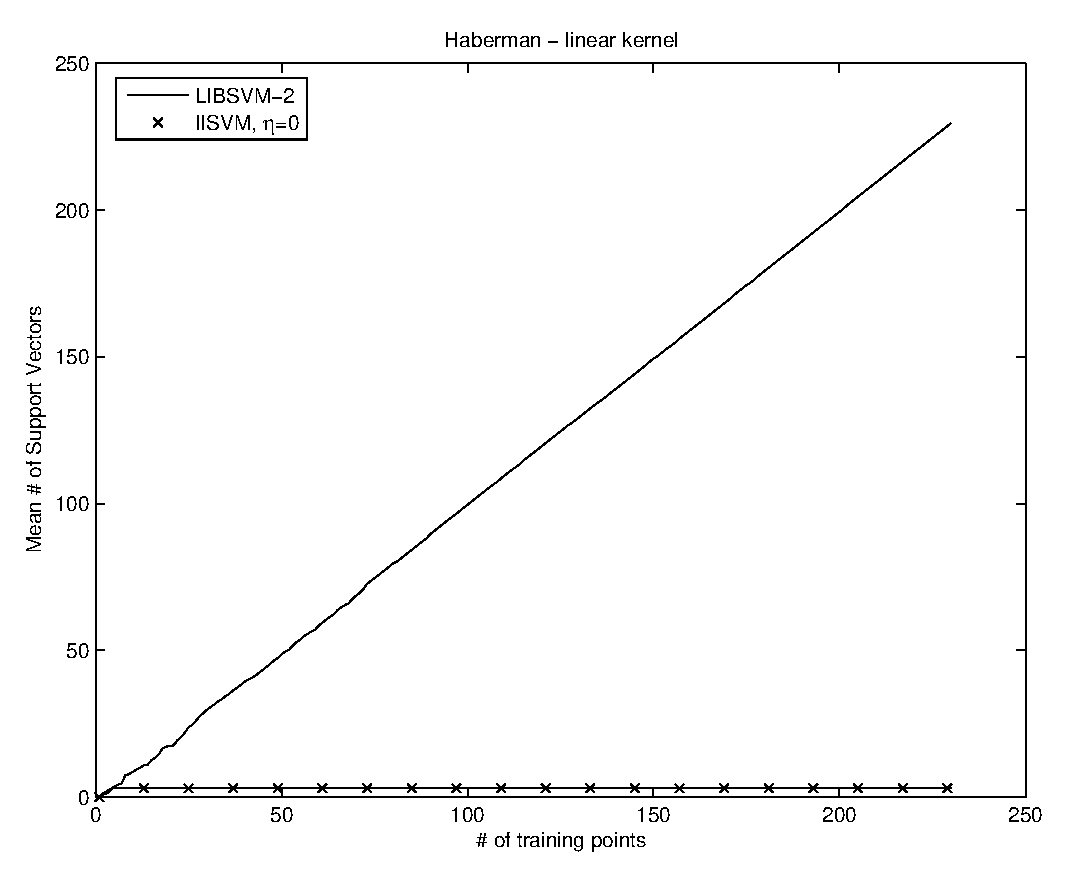
\includegraphics[width=0.45\textwidth]{Haberman_lin} &
       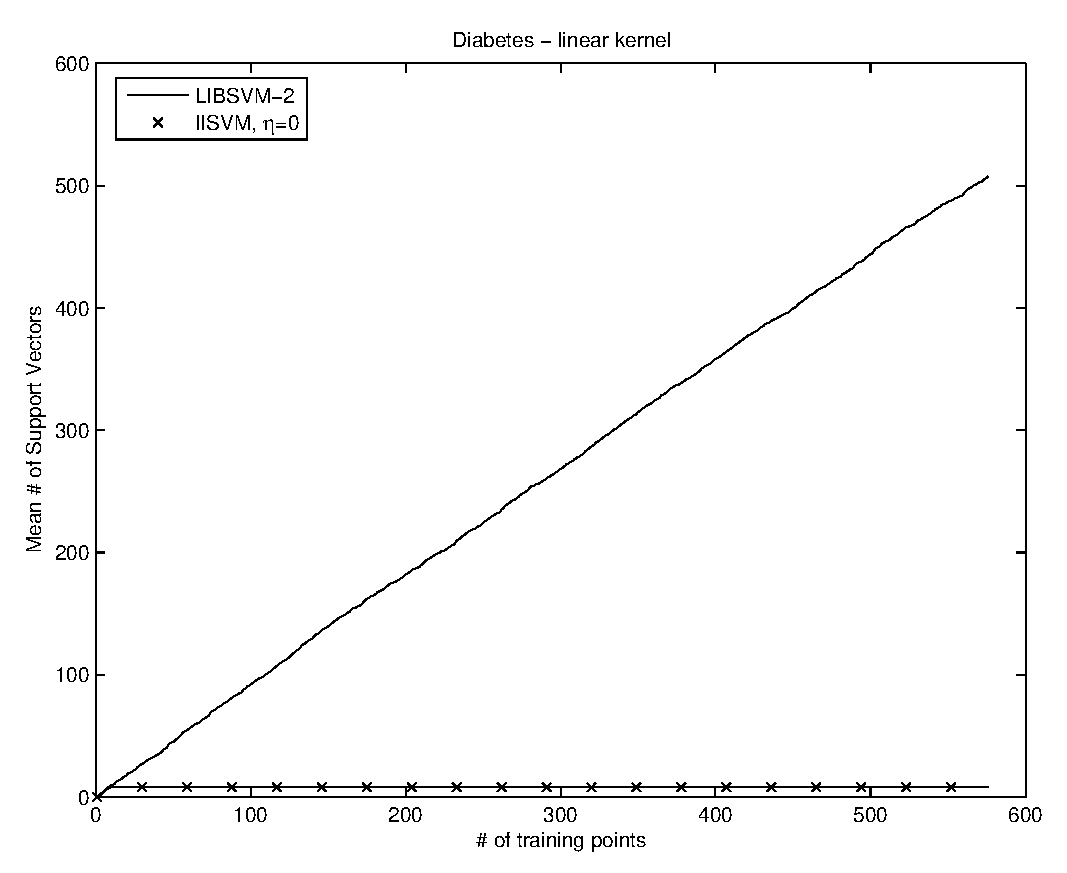
\includegraphics[width=0.45\textwidth]{Diabetes_lin} \\
       \multicolumn{2}{c}{(a)} \\
       \includegraphics[width=0.45\textwidth]{Haberman_poly3} &
       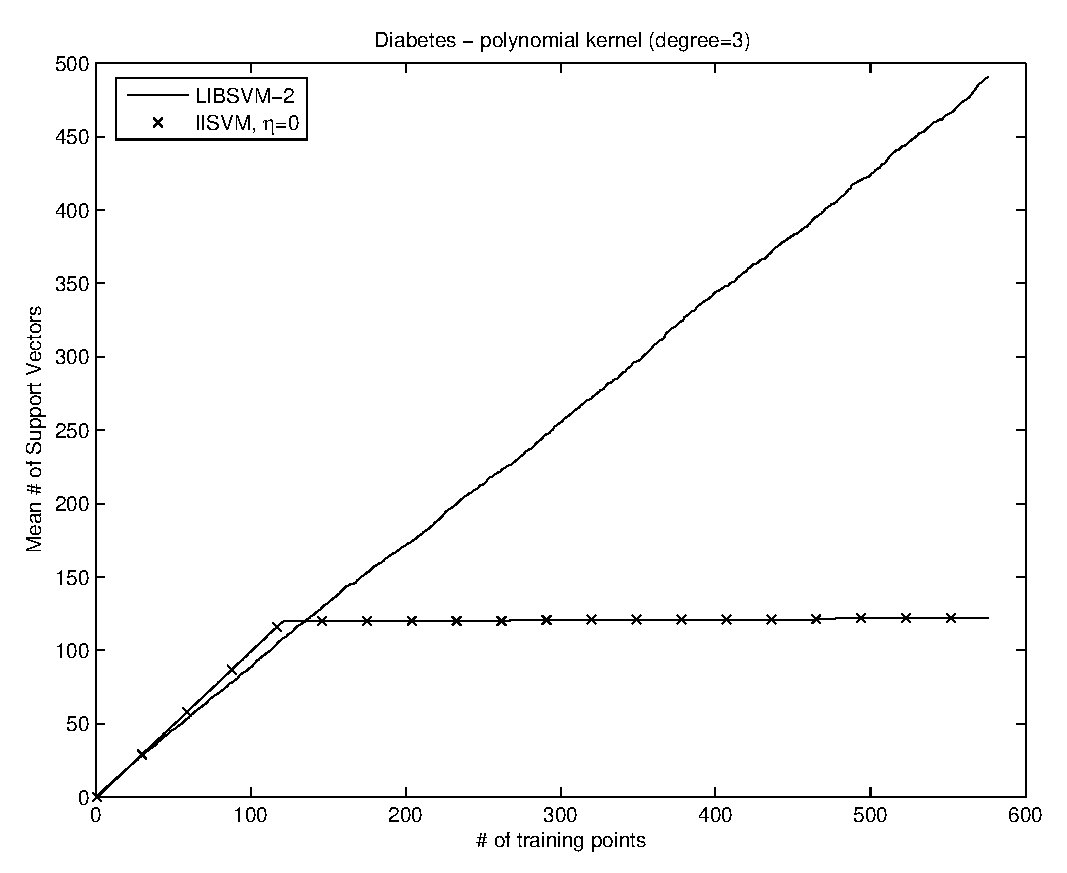
\includegraphics[width=0.45\textwidth]{Diabetes_poly3} \\
       \multicolumn{2}{c}{(b)} \\
    \end{tabular}
  \end{center}
  \caption{\label{fig:finite} test results with finite-dimensional
  kernels: (a) linear kernel, (b) polynomial kernel with degree $3$.}
\end{figure*}

\begin{figure*}[!htbp]
  \begin{center}
    \begin{tabular}{cc}
       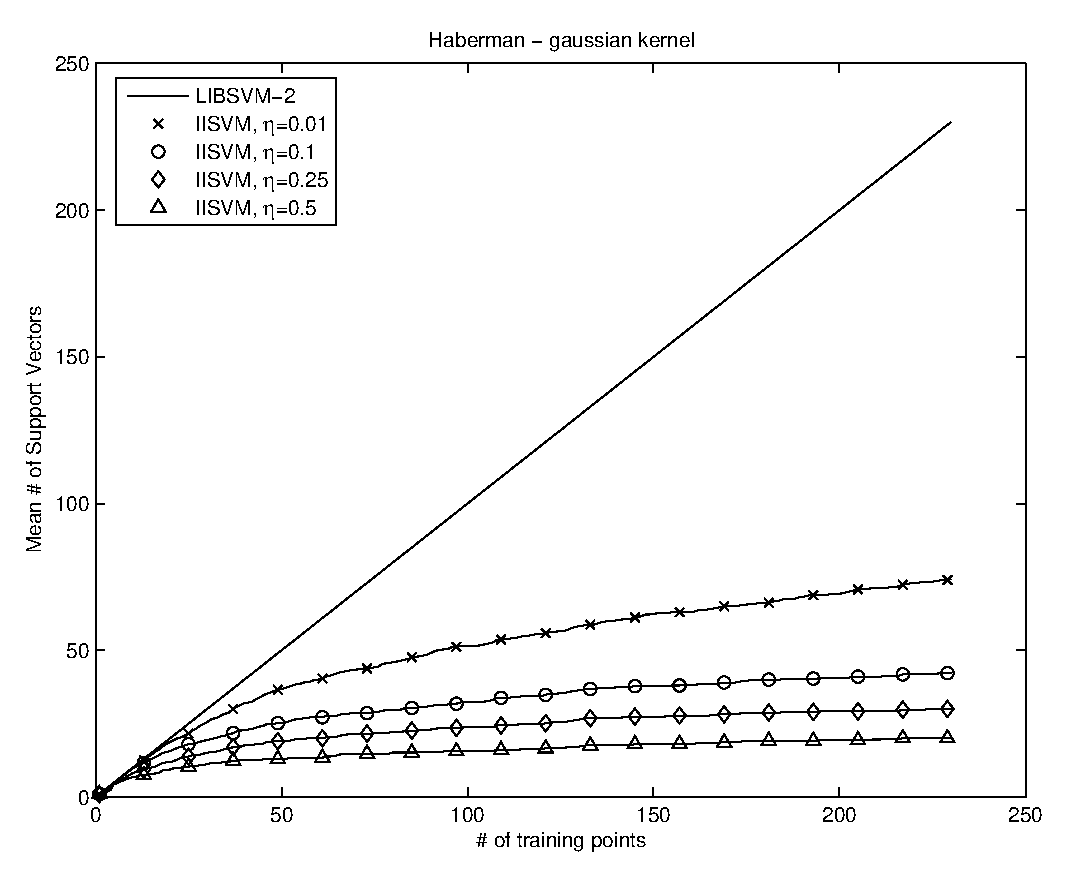
\includegraphics[width=0.45\textwidth]{Haberman_gaussian} &
       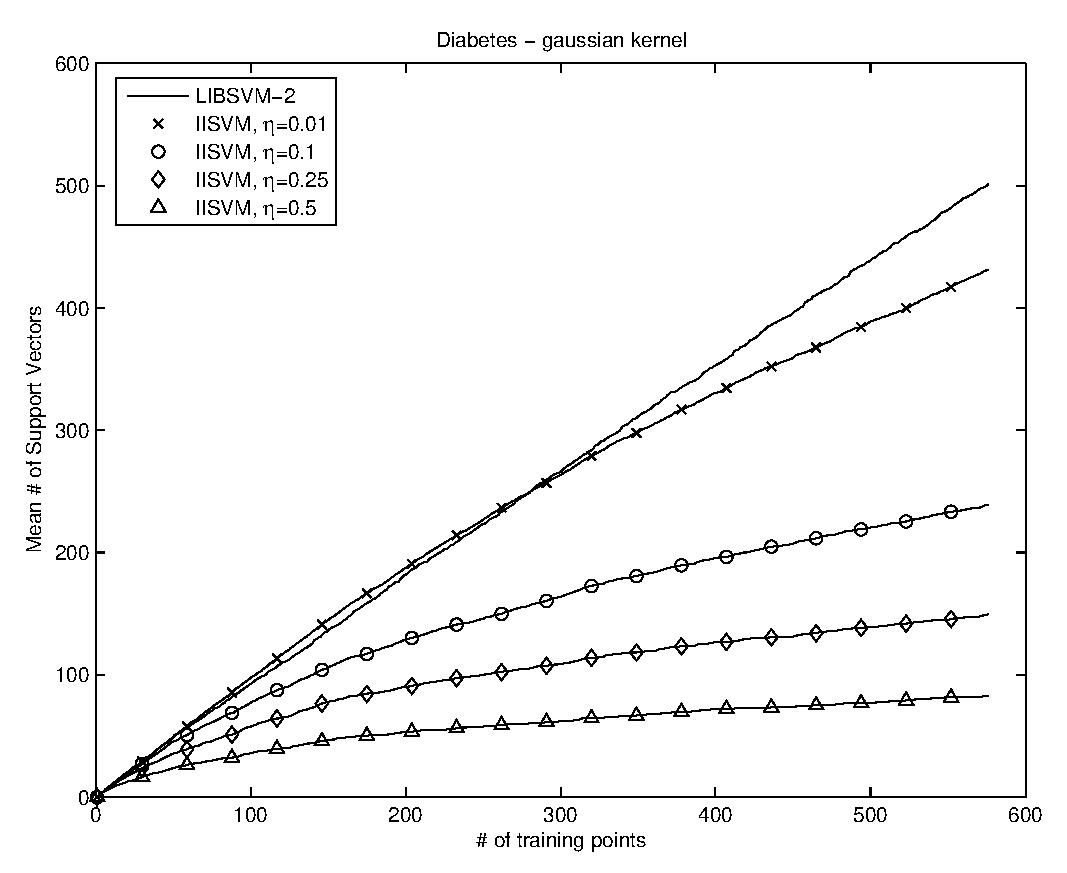
\includegraphics[width=0.45\textwidth]{Diabetes_gaussian}
    \end{tabular}
  \end{center}
  \caption{\label{fig:infinite} test results with an infinite-dimensional
  (Gaussian) kernel.}
\end{figure*}

Consider Figure \ref{fig:finite}: as one can see, as opposed to the
linear behaviour of LIBSVM-2, IISVMs quickly attain a constant number
of support vectors and then stop acquiring new ones. The values are,
in turn, $3$ support vectors in Figure \ref{fig:finite}(a) and $10$
and $120$ in Figure \ref{fig:finite}(b). These numbers match exactly
the dimensions of the related feature spaces, given by
$\binom{m+deg-1}{deg}$ where $deg$ is the degree of the polynomial
kernel (obviously $1$ in the case of linear kernels).

Consider Figure \ref{fig:infinite}: in this case IISVMs obtains a
dramatic reduction in the number of support vectors, as expected, as
the tolerance threshold $\eta$ is made larger and larger. Also, the
shape of the curve seems in most cases to be no longer linear but
rather somehow logarithmic. As $\eta$ is raised, as expected, the
relative error\footnote{let $e$ and $e'$ be the error obtained
in turn by IISVM and LIBSVM-2; then the relative error is defined as
$(e'-e)/e'$.} with respect to LIBSVM-2 grows, but
in a remarkably small way: in the worst cases, that is for $\eta=0.5$,
the relative error is slightly more than $1\%$ with respect to
LIBSVM-2, whereas it is $0.24\%$ for the Haberman suite.

As a final remark, notice that in general the number of support
vectors chosen by IISVMs could be higher than that obtained by
SVMs. An example of this phenomenon is visible in Figure
\ref{fig:infinite}, right plot, between x-values $100$ and $200$.



%%%%%%%%%%%%%%%%%%%%%%%%%%%%%%%%%%%%%%%
\section{Conclusions}
\label{sec:concl}
%%%%%%%%%%%%%%%%%%%%%%%%%%%%%%%%%%%%%%%%
We presented a new method to reduce the number of SVs needed by a
Support Vector Machine in an online setting, called OISVMs (Online
Independent Support Vector Machines). OISVMs avoid using in the
solution those support vectors which are linearly dependent of
previous ones in the feature space --- in other words, the kernel
matrix is always kept at full rank. The optimization problem is solved
via an incremental algorithm which benefits of the small size of the
kernel matrix.

We tested the method both on a standard set of benchmark databases and
a real-world case study, namely place recognition in an indoor
environment, from sequences acquired by robot platforms under
different weather conditions and across a time span of several months.

The experimental results show that $(i)$ in the case of
finite-dimensional kernels, OISVMs attain the theoretical limit of
linearly independent support vectors allowed by the feature space,
without losing any accuracy with respect to ordinary SVMs; $(ii)$ in
the case of infinite-dimensional kernels, they dramatically reduce the
number of support vectors at the price of a negligible degradation in
the accuracy. In fact, OISVMs obtain an accuracy up to $0.063\%$ worse
than SVMs with less than $5\%$ of the support vectors of a standard
SVM on a set of standard benchmark databases; whereas, on the
real-world application, we get as few as one third of the SVs required
by the fixed-partition method, while retaining essentially the same
accuracy.

A current limitation of the algorithm is that it requires to store in
memory all training data. This is unfeasible for applications like
place recognition by robot platforms, as it might lead to a memory
explosion. A possible solution might be to combine the OISVM with the
KNN-SVM algorithm \cite{zhang:cvpr06}, so to keep separated the data
storage from the discriminative classification. Another possibility is
to discard training data in a principled way, so to minimize the
effect on the SV solution. Future work will focus on this issue.



% ------------------------------------------------------------------------ 

{\small
\bibliographystyle{ieee}
\bibliography{paper}
}

\end{document}
